\documentclass[10pt]{article}
\usepackage[utf8]{inputenc}
\usepackage{listings}
\usepackage{float}
\usepackage{graphicx}
\usepackage{fullpage}
\usepackage{caption}
\usepackage{subcaption}
\usepackage{amsmath}
\usepackage{hyperref}

%\renewcommand{\thesubsection}{\arabic{subsection}}
\renewcommand{\thesubsubsection}{\alph{subsubsection}}

\title{Pattern Recognition Practical 4}
\author{Group 24: \and Maikel Withagen (s1867733) \and Steven Bosch (s1861948)}
\date{\today}
\lstset{
frame=single, 
numbers=left, 
breaklines=true, 
language=Matlab,
basicstyle=\footnotesize, 
title=\lstname,
showstringspaces=false
}

\renewcommand{\thesection}{Assignment \arabic{section}}
\renewcommand{\thesubsection}{\arabic{subsection}}
\begin{document}
\maketitle

\section{Supervised learning: LVQ1}
Using the code given in the appendix(\autoref{code1_1}) we created the scatterplot in figure \ref{fig1.1}.

\begin{figure}[H]
 \centering
 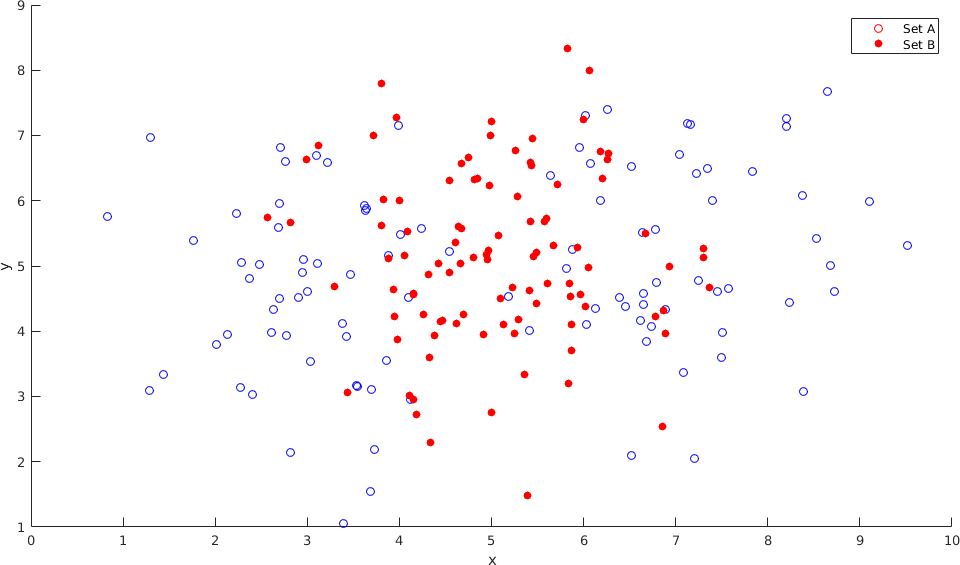
\includegraphics[width=\textwidth]{Fig1_1.png}
 \caption{Scatterplot for the two classes.}
 \label{fig1.1}
\end{figure}

The plot shows that there are at least three prototypes needed to approach a fairly well classification of these data. Two for set A, which should probably be located around $(3,4.5)$ and $(7.5, 5.5)$, and one for set B somewhere around $(5,5)$. 

\subsection{}
The code in the appendix(\autoref{code1_2}) shows our implementation of the LVQ1 algorithm. We acquired the following results for the different settings.

\subsubsection{1 Prototype for class A and 1 prototype for class B}

\begin{figure}[H]
 \centering
 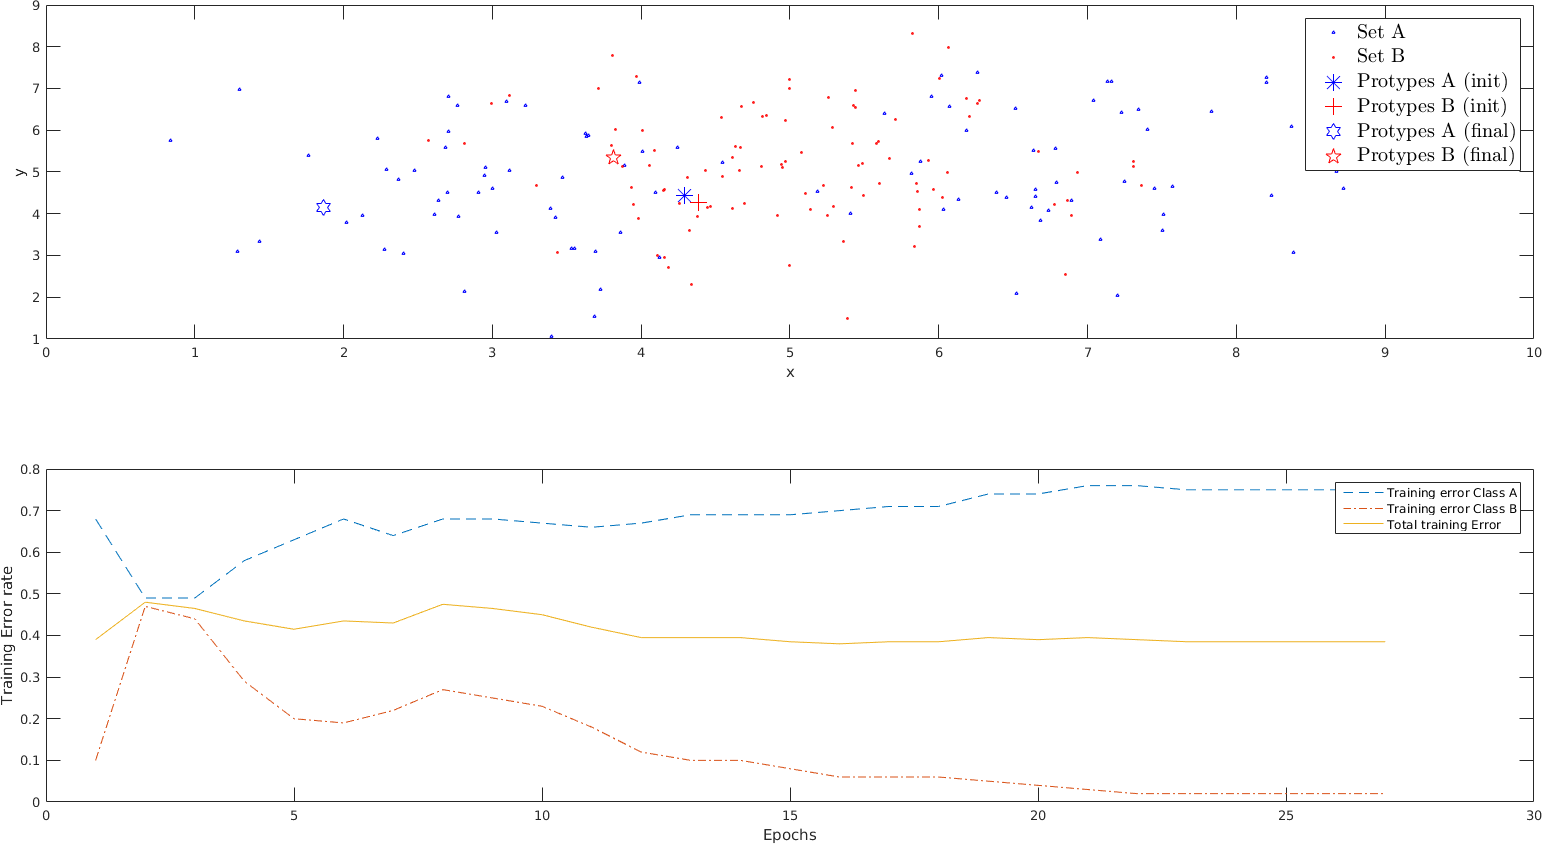
\includegraphics[width=\textwidth]{Fig12_a1.png}
 \caption{Classification for 1 prototype for class A and 1 prototype for class B. Plot two gives the corresponding error rates (Class 1 is A and class 2 is B).}
 \label{fig1.12a}
\end{figure}
As is expected with only one prototype per class, figure \ref{fig1.12a} shows that the prototype for class B is formed quite well, allowing it to correctly classify at least the data points that belong to class B (an error stabilising at around 0.03). However, since class A is distributed in two groups, with B in between them, the prototype for class A is formed at of one of the two outer clusters, which means it can only correctly classify a part of that cluster correctly. The other cluster will be incorrectly classified as belonging to class B, which follows from its error rate which stabilises at around 0.77, meaning that on average 77 out of 100 data points are incorrectly classified, which is quite high. Ultimately this results in a total error rate that stabilises at around 0.4.

\subsubsection{1 Prototype for class A and 2 prototype for class B}

\begin{figure}[H]
 \centering
 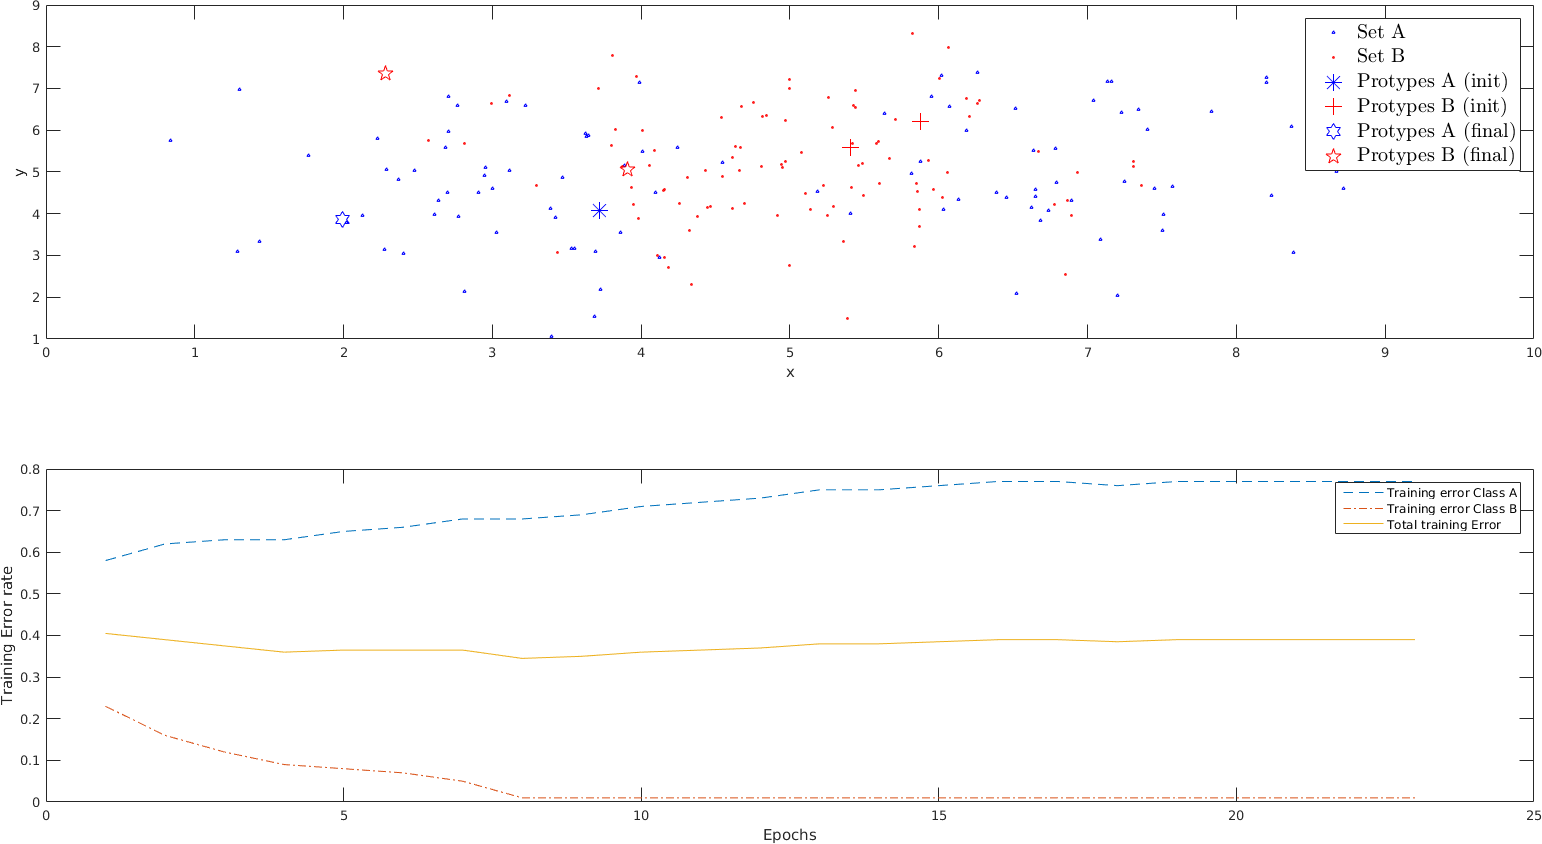
\includegraphics[width=\textwidth]{Fig12_b.png}
 \caption{Classification for 1 prototype for class A and 2 prototypes for class B. Plot two gives the corresponding error rates (Class 1 is A and class 2 is B).}
 \label{fig1.12b}
\end{figure}
In this case figure \ref{fig1.12b} shows the same thing happening with the prototype for class A: it ends up in one of the two separated A-clusters. Its error is therefore also similar to that in the previous case. On the other hand we see that the two prototypes for class B, even though the data points belonging to class B are clustered in one big cluster, we see that a second prototype slightly improves the result, giving an error that stabilises near 0. This might be the case because it `catches' some of the last data points that were mixed in with the left-side class A cluster, meaning that it also causes some of the class-B data points in that cluster to be misclassified. This explains the fact that the error of class A has become slightly higher, resulting in a total error that is approximately the same as in the previous case.

\subsubsection{2 Prototype for class A and 1 prototype for class B}

\begin{figure}[H]
 \centering
 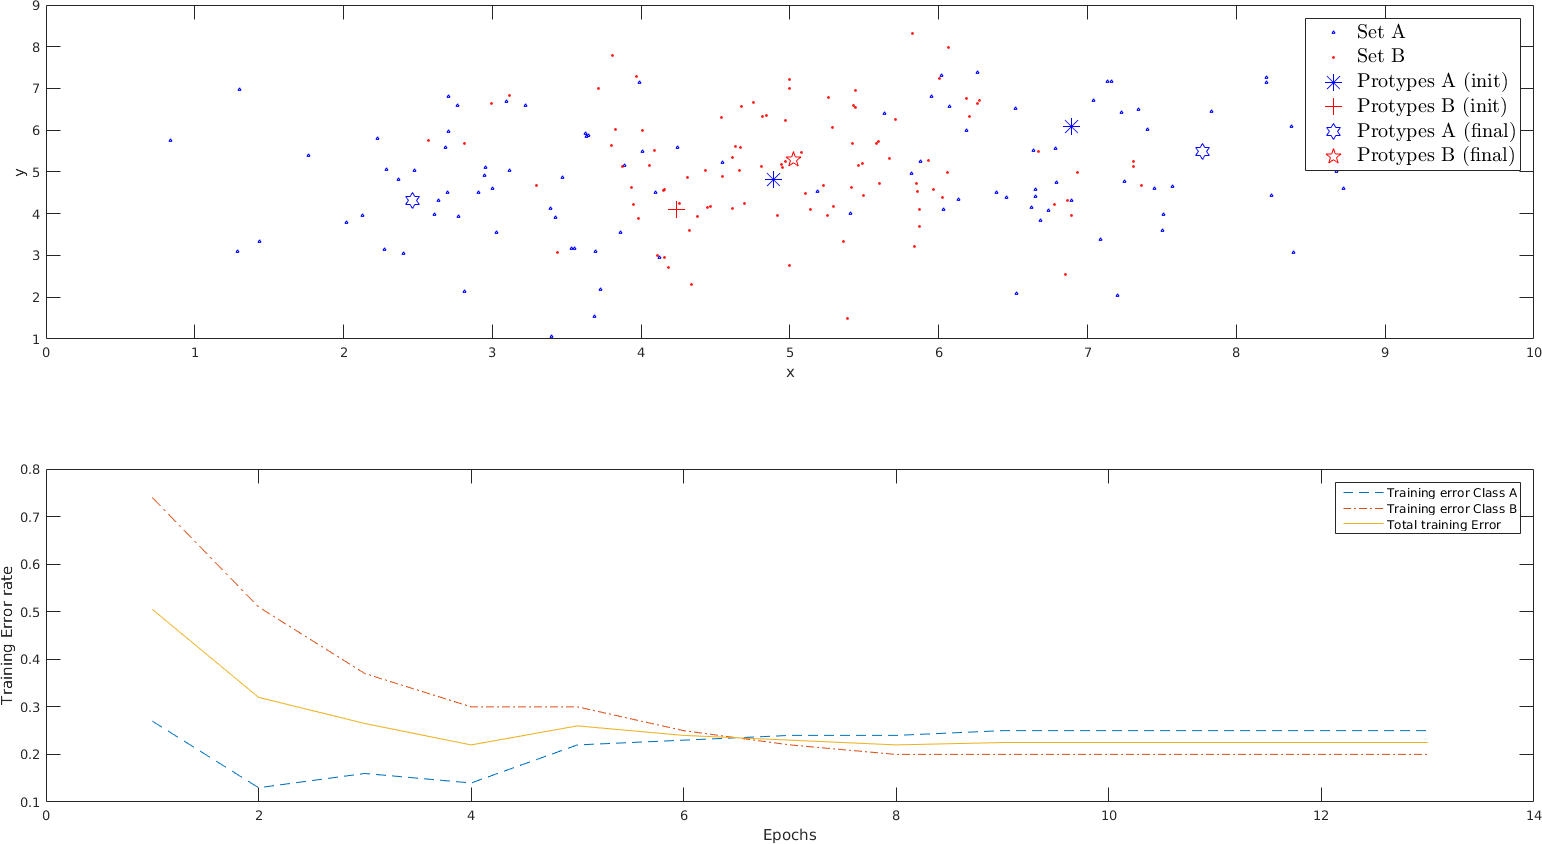
\includegraphics[width=\textwidth]{Fig12_c.png}
 \caption{Classification for 2 prototypes for class A and 1 prototype for class B. Plot two gives the corresponding error rates (Class 1 is A and class 2 is B).}
 \label{fig1.12c}
\end{figure}
In this case figure \ref{fig1.12c} shows a much lower error rate than in the previous two cases. This is due to the fact that there are now two prototypes for class A, which can classify the seperated data points much better, since they are grouped into two clusters (one prototype for the left cluster, one for the right). Ultimately this results in a total error that stabilises around 0.22, which is significantly lower than in the previous two cases. However, there are also cases in which this amount of prototypes does not result in this error rate. This is the case when the initialization is such that both prototypes for class A begin somewhere near the same cluster of class A, meaning that they will never get to the other cluster, because they get `pushed away' by the data points belonging to class B. In such a case the result yields about the same error rate as the case discussed in the previous paragraph.

\subsubsection{2 Prototype for class A and 2 prototype for class B}

\begin{figure}[H]
 \centering
 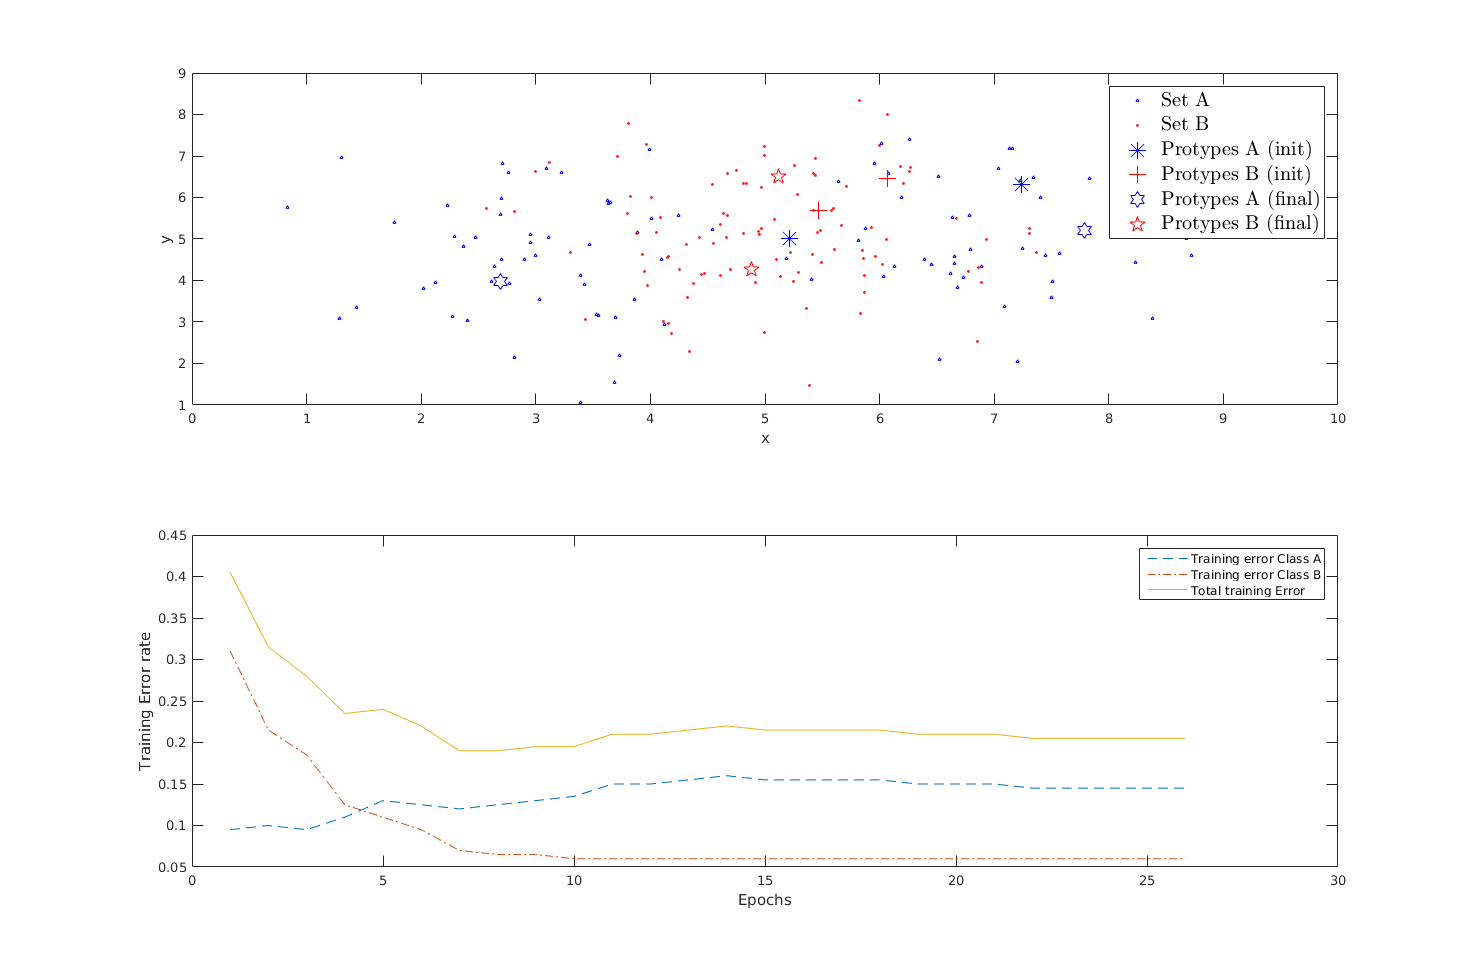
\includegraphics[width=\textwidth]{Fig12_d.png}
 \caption{Classification for 2 prototypes for class A and 2 prototypes for class B. Plot two gives the corresponding error rates (Class 1 is A and class 2 is B).}
 \label{fig1.12d}
\end{figure}
Finally in the case of two prototypes for each class, figure \ref{fig1.12d} shows slightly worse results than for the previous case, with a total error stabilising at approximately 0.23. This has probably to do with the two prototypes for class B now being divided over the one cluster of data points, which causes them to be slightly nearer to the data points that belong to class A. This causes some of those data points to be misclassified, resulting in a slightly higher error.

\bigskip
\noindent Overall we can state that the case for two prototypes for class A and one for class B yields the best results for this particular data set. This is of course also the intuitve explanation, since any human can immediately see that the clusters are distributed in such a way that this distribution of prototypes is needed.

\subsubsection{Learning rate}
To investigate the influence of the learning rate, we've run a simulation with a higher, and a lower learning rate, 
both with the same parameters as Assignment 1c.
\begin{figure}[H]
 \centering
 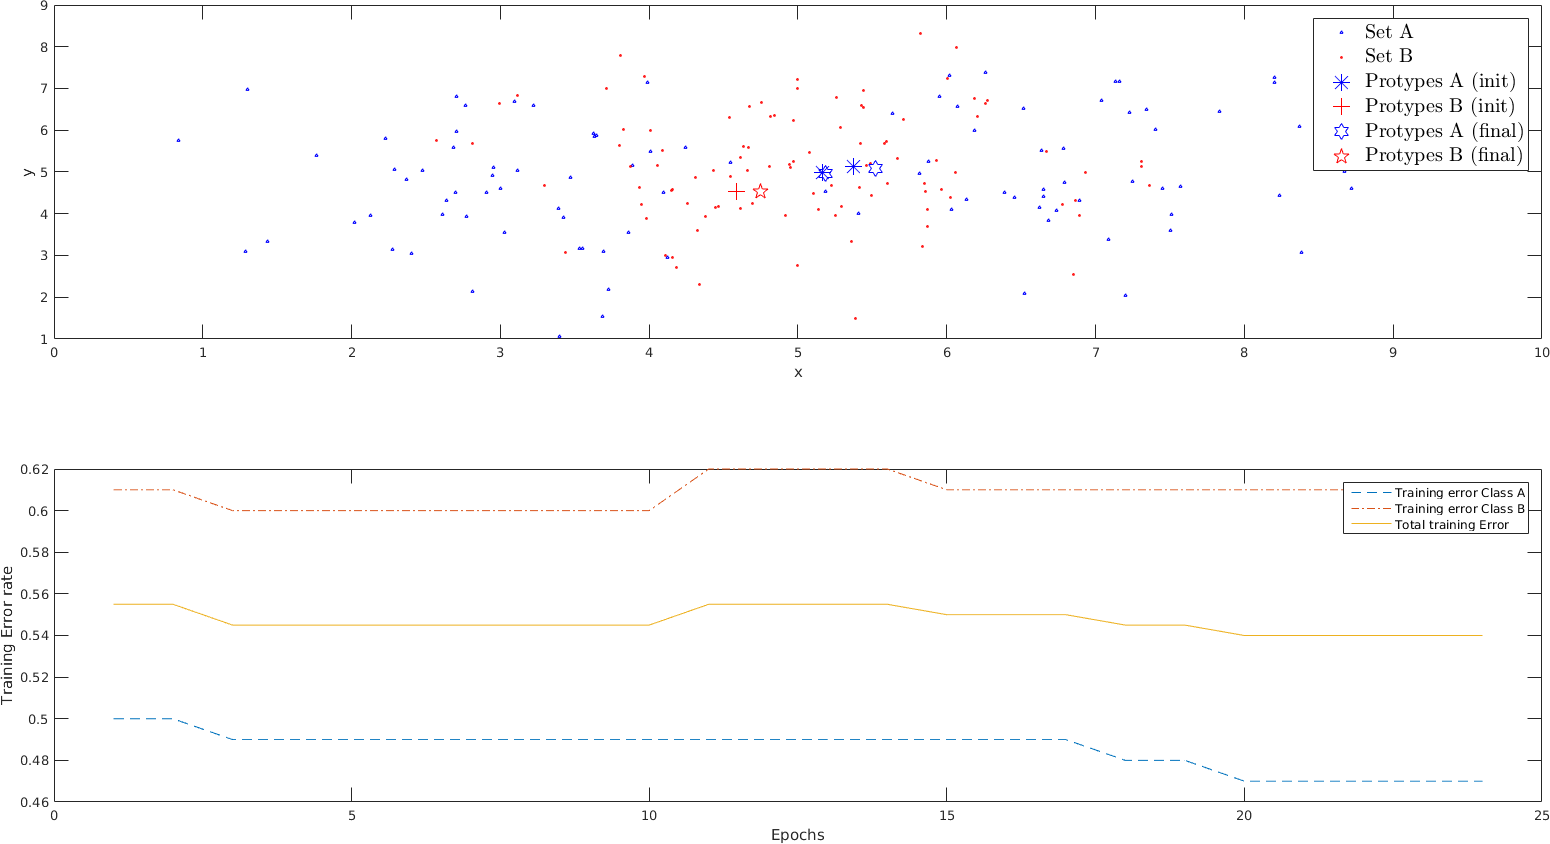
\includegraphics[width=\textwidth]{Fig12_c_0001.png}
 \caption{Classification as Assignment 1c, with $\eta=0.0001$}
 \label{fig1.12c_0001}
\end{figure}
Figure \ref{fig1.12c_0001} shows a simulation with $\eta=0.0001$. The prototype positions and the error rate 
both suggest that the algorithm was unable to classify with the same performance as simulations with a higher error rate.
The error value do have stabilized, so it seems that lowering the learning rate ``decreases'' the pull that the data points have 
on the prototypes, resulting in non-optimal results with most likely local-optimal positions for the prototypes.

\begin{figure}[H]
 \centering
 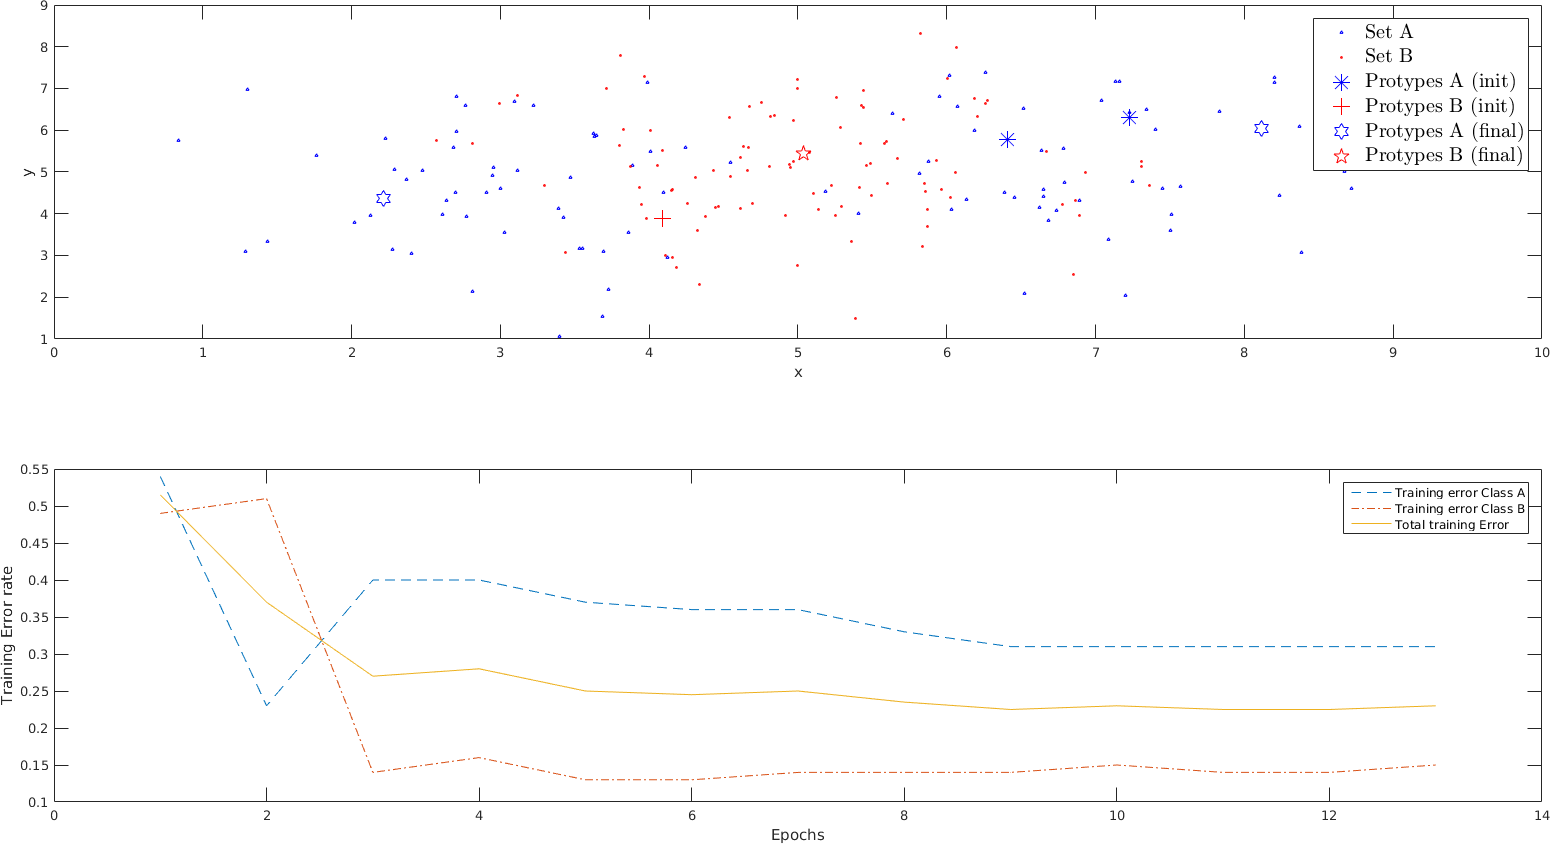
\includegraphics[width=\textwidth]{Fig12_c_03.png}
 \caption{Classification as Assignment 1c, with $\eta=0.03$}
 \label{fig1.12c_03}
\end{figure}

Figure \ref{fig1.12c_03} shows a simulation with $\eta=0.03$, only slightly higher then the default value.
This higher learning rate causing to points to ``pull'' harder on the prototypes. 
Even for this slight increase in learning rate, we had to decrease our stopping-threshold by a ten-fold, since the prototype positions did not stabilize.

In conclusion, we can say that the learning rate in LVQ1 corresponds to the strength of the ``pull'' that data points have on the prototype positions.
If this pull is too strong, the prototype positions do not stabilize and will hover around their optimal positions.
If this pull is too weak, the data points are unable to attract the prototypes to their optimal positions and 
the prototypes might end up in local, but not the optimal, optima positions.



\section{Cross validation}
The code in the appendix(\autoref{code2}) gives our implementation for this assignment. The computed mean of the 10 values of the classification error is 0.300. This is slightly higher than the error rates that were yielded in assignment 1.2(c), which ended up at a total error of around 0.22. 
It is worth mentioning that certain subsets yielded a high error rate in multiple experiments.
This might suggest that the points in these subsets are important for correct training of the prototypes.

\section{Relevance LVQ}
The code in the appendix(\autoref{code3a}) has produced the following image:
\begin{figure}[H]
 \centering
 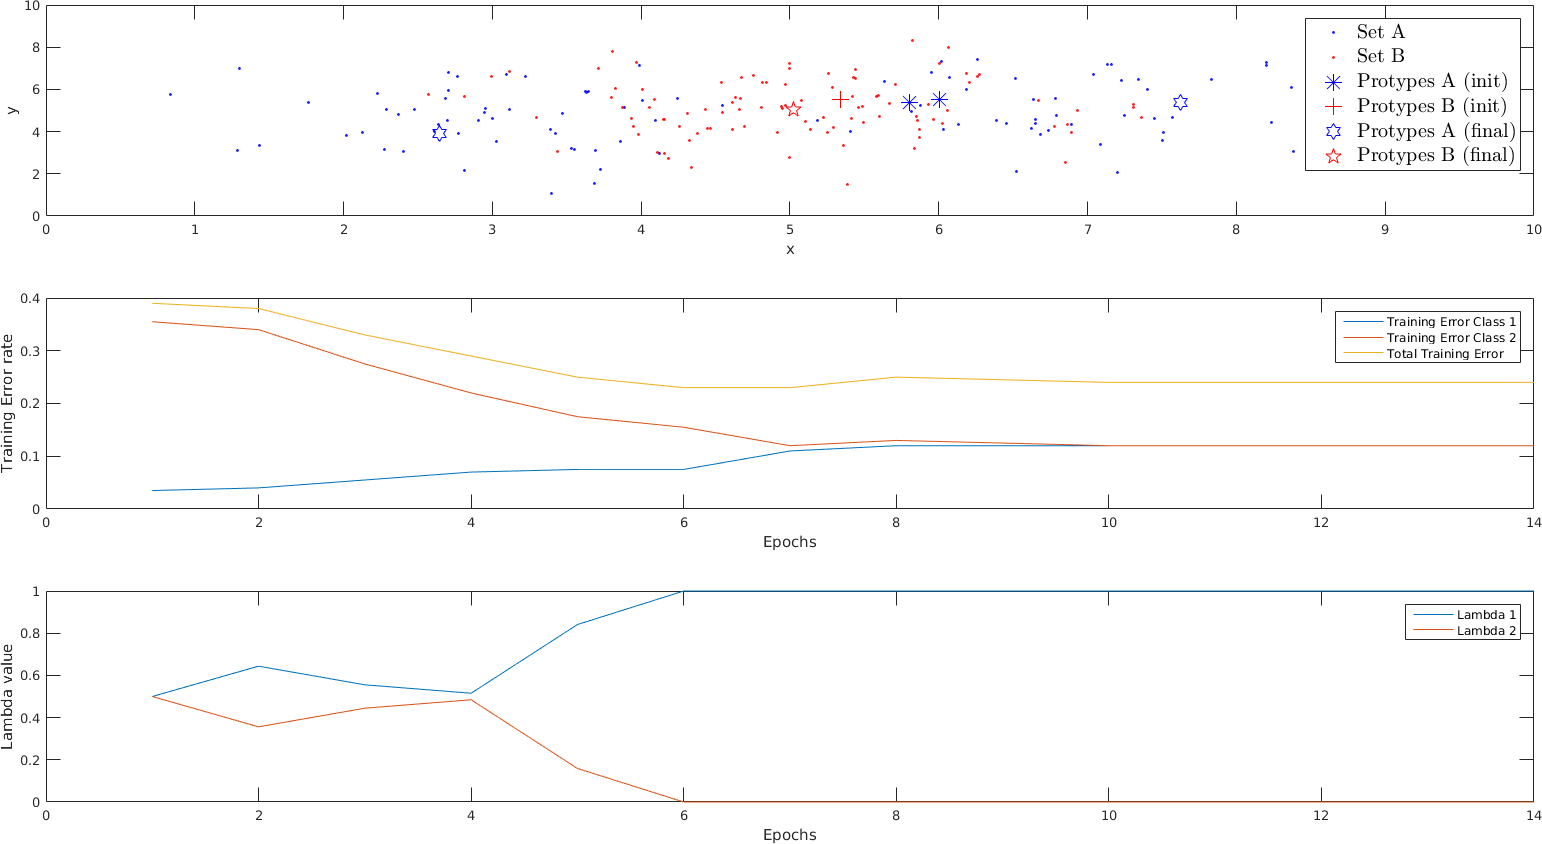
\includegraphics[width=\textwidth]{Fig3a.png}
 \caption{}
 \label{fig3a}
\end{figure}

Looking at the final prototypes in \autoref{fig3a}, we can see that their final positions are similar to ones we saw in earlier assignments.
The final error rate also lies around the same value as earlier.
This suggests that the prototypes are able to classify with the same performance as in earlier assignments.
However, an interesting difference is the learning speed of the algorithm. 
By using a Relevance LVQ, the error rates have stabilized after only $\approx15$ epochs, which is less then earlier results.
The learning curves for the relevances show a mirrorlike behavior due to the mandatory normalization step.
Interesting to see is that after some initial movement, their values want to fan out (as was observed in experiments where the normalization step was skipped).
This fanning out in combination with the normalization step results in two bottom/ceiling values for the learning values (i.e.\ 1.0 and 0.0),
effectively further adjusting the prototypes only on a single dimension.
This can be explained by the fact that the ``separation'' lines for the two data set are two vertical lines, 
so once the prototypes have acquired the correct vertical value (i.e.\ the y-value, learned with lambda 2),
only corrections in the x-values (i.e.\ lambda 1) are neccesary.

The improvement of this algorithm can also be observed in the K-fold estimation test error, 
which is $0.0250$, as calculated with the code in the appendix(\autoref{code3b}.
This value is lower than with the regular LVQ1 algorithm, suggesting that Relevance LVQ has learned to classify even better than LVQ1.
\newpage
\section*{Appendix}
\subsection{Code 1.1}
\lstinputlisting{../Code/Ass1_1.m}{\label{code1_1}}
\subsection{Code 1.2}
\lstinputlisting{../Code/Ass1_2.m}{\label{code1_2}}
\subsection{Code 2}
\lstinputlisting{../Code/Ass2.m}{\label{code2}}
\subsection{Code 3a}
\lstinputlisting{../Code/Ass3.m}{\label{code3a}}
\subsection{Code 3b}
\lstinputlisting{../Code/Ass3.m}{\label{code3b}}



\maketitle
\end{document}
